%%
%% Beginning of file 'sample.tex'
%%
%% Modified 2005 December 5
%%
%% This is a sample manuscript marked up using the
%% AASTeX v5.x LaTeX 2e macros.

%% The first piece of markup in an AASTeX v5.x document
%% is the \documentclass command. LaTeX will ignore
%% any data that comes before this command.

%% The command below calls the preprint style
%% which will produce a one-column, single-spaced document.
%% Examples of commands for other substyles follow. Use
%% whichever is most appropriate for your purposes.
%%
%\documentclass[12pt,preprint]{aastex}

%% manuscript produces a one-column, double-spaced document:

%\documentclass[manuscript]{aastex}
%\documentclass[onecolumn]{emulateapj}

%% preprint2 produces a double-column, single-spaced document:

 \documentclass[preprint2]{aastex}

%% Sometimes a paper's abstract is too long to fit on the
%% title page in preprint2 mode. When that is the case,
%% use the longabstract style option.

%% \documentclass[preprint2,longabstract]{aastex}

%% If you want to create your own macros, you can do so
%% using \newcommand. Your macros should appear before
%% the \begin{document} command.
%%
%% If you are submitting to a journal that translates manuscripts
%% into SGML, you need to follow certain guidelines when preparing
%% your macros. See the AASTeX v5.x Author Guide
%% for information.

\newcommand{\vdag}{(v)^\dagger}
\newcommand{\myemail}{jbyrne@ifa.hawaii.edu}

%%I'm adding these -JPB
\usepackage{subfigure}
%\newcommand{\solphys}{{\it Solar Physics}}
%\newcommand{\aap}{    {\it Astronomy \& Astrophysics}}
%\newcommand{\aaps}{   {\it Astronomy \& Astrophysics Supplemental}}
%\newcommand{\apj}{    {\it Astrophysical Journal}}
%\newcommand{\apjl}{    {\it Astrophysical Journal Letters}}
%\newcommand{\jgr}{    {\it Journal of Geophysical Research}}
%\newcommand{\aapr}{    {\it Astronomy \& Astrophysics Review}}
%\newcommand{\grl}{    {\it Geophysical Research Letters}}
\newcommand{\lrsp}{    {\it Living Rev. Solar Phys.}}

\newcommand{\RNum}[1]{\uppercase\expandafter{\romannumeral #1\relax}}

%\makeatletter
%\newcommand*{\rom}[1]{\expandafter\@slowromancap\romannumeral #1@}
%\makeatother

%% You can insert a short comment on the title page using the command below.

\slugcomment{Paper \RNum{2} of \RNum{2}}

%% If you wish, you may supply running head information, although
%% this information may be modified by the editorial offices.
%% The left head contains a list of authors,
%% usually a maximum of three (otherwise use et al.).  The right
%% head is a modified title of up to roughly 44 characters.
%% Running heads will not print in the manuscript style.

\shorttitle{Interesting event 2011-03-08}
\shortauthors{Byrne et al.}

%% This is the end of the preamble.  Indicate the beginning of the
%% paper itself with \begin{document}.

\begin{document}

%% LaTeX will automatically break titles if they run longer than
%% one line. However, you may use \\ to force a line break if
%% you desire.

\title{Investigating the 2011-03-08 eruption}

%% Use \author, \affil, and the \and command to format
%% author and affiliation information.
%% Note that \email has replaced the old \authoremail command
%% from AASTeX v4.0. You can use \email to mark an email address
%% anywhere in the paper, not just in the front matter.
%% As in the title, use \\ to force line breaks.

\author{J. P. Byrne$^1$ et al.} %, D. Seaton$^2$, H. Morgan$^{3,1}$, S. R. Habbal$^1$
\affil{$^1$Institute for Astronomy, University of Hawai'i, 2680 Woodlawn Drive, Honolulu, HI 96822, USA.}
%\affil{$^3$Institute of Mathematics and Physics, Aberystwyth University, Ceredigion, Wales, SY23 3BZ.}

\email{jbyrne@ifa.hawaii.edu}

%% Notice that each of these authors has alternate affiliations, which
%% are identified by the \altaffilmark after each name.  Specify alternate
%% affiliation information with \altaffiltext, with one command per each
%% affiliation.


%% Mark off your abstract in the ``abstract'' environment. In the manuscript
%% style, abstract will output a Received/Accepted line after the
%% title and affiliation information. No date will appear since the author
%% does not have this information. The dates will be filled in by the
%% editorial office after submission.

\begin{abstract}
Methods of multiscale image analysis were employed and their efficacy on the SWAP data tested for revealing CME structure while suppressing other features. The methods employed are described in detail in \citet{2008SoPh..248..457Y}, whereby successive filtering of an image via a Gaussian and derivative-of-Gaussian produces a number of scales of detail to be inspected. This also produces an image with intensities that represent the relative edge strengths in the original image, which can be used to characterize the structure of interest -- specifically for this case the erupting material involved in the CME. In order to overlap the observations from SWAP and MK4, the core material of the CME in its early eruption phase was chosen for its higher signal to noise ratio than the CME front, for example, that was not discernible in the early stages of the observations. In the LASCO field-of-view, the core material was determined to be moving at the same speed as the CME front, at $\sim500~km~s^{-1}$. The front portion of the core material in the MK4 images was characterized via point-\&-click methodology on the multiscale images of enhanced edges, and an ellipse was fit to the curved front. The same was done for the erupting loop structure observed in SWAP, with the expectation that it might directly correlate to the CME core. However, it was found that the erupting material that starts at the same time and location in both the MK4 and SWAP images, did not proceed to erupt at the same rate. Rather the core material observed in MK4 moves at greater speeds than the loop structures observed in SWAP; rising from an initial speed of $\sim100~km~s^{-1}$ (at $\sim1.5~R_{\odot}$) to a final speed of $\sim400~km~s^{-1}$ (at $\sim2~R_{\odot}$), while the loops continue to steadily rise at $\sim100~km~s^{-1}$. The reason for this is unclear, and requires further investigation.
\end{abstract}


%% Keywords should appear after the \end{abstract} command. The uncommented
%% example has been keyed in ApJ style. See the instructions to authors
%% for the journal to which you are submitting your paper to determine
%% what keyword punctuation is appropriate.

\keywords{Sun: activity; Sun: corona; Sun: coronal mass ejections (CMEs); Techniques: image processing}

%% From the front matter, we move on to the body of the paper.
%% In the first two sections, notice the use of the natbib \citep
%% and \citet commands to identify citations.  The citations are
%% tied to the reference list via symbolic KEYs. The KEY corresponds
%% to the KEY in the \bibitem in the reference list below. We have
%% chosen the first three characters of the first author's name plus
%% the last two numeral of the year of publication as our KEY for
%% each reference.


%% Authors who wish to have the most important objects in their paper
%% linked in the electronic edition to a data center may do so by tagging
%% their objects with \objectname{} or \object{}.  Each macro takes the
%% object name as its required argument. The optional, square-bracket 
%% argument should be used in cases where the data center identification
%% differs from what is to be printed in the paper.  The text appearing 
%% in curly braces is what will appear in print in the published paper. 
%% If the object name is recognized by the data centers, it will be linked
%% in the electronic edition to the object data available at the data centers  
%%
%% Note that for sources with brackets in their names, e.g. [WEG2004] 14h-090,
%% the brackets must be escaped with backslashes when used in the first
%% square-bracket argument, for instance, \object[\[WEG2004\] 14h-090]{90}).
%%  Otherwise, LaTeX will issue an error. 

\section{Introduction}

An important aspect of studying CMEs, is the ability to resolve their low-corona propagation and associated source regions on the disk; be it a flaring or non-flaring active region, a prominence/filament eruption or other rising loop system, or else a `stealth CME' without any specifically detectable source. Prominence lift-offs often become the core material of a CME, and rising loops often form some part of the CME morphology. Their low-corona kinematics and morphology provide insight into the early forces at play, and so a rigorous study of such phenomena is key to understanding the physics involved in the initiation phase of CMEs.

\section{Techniques}

%\begin{figure}[!ht]
%\centering{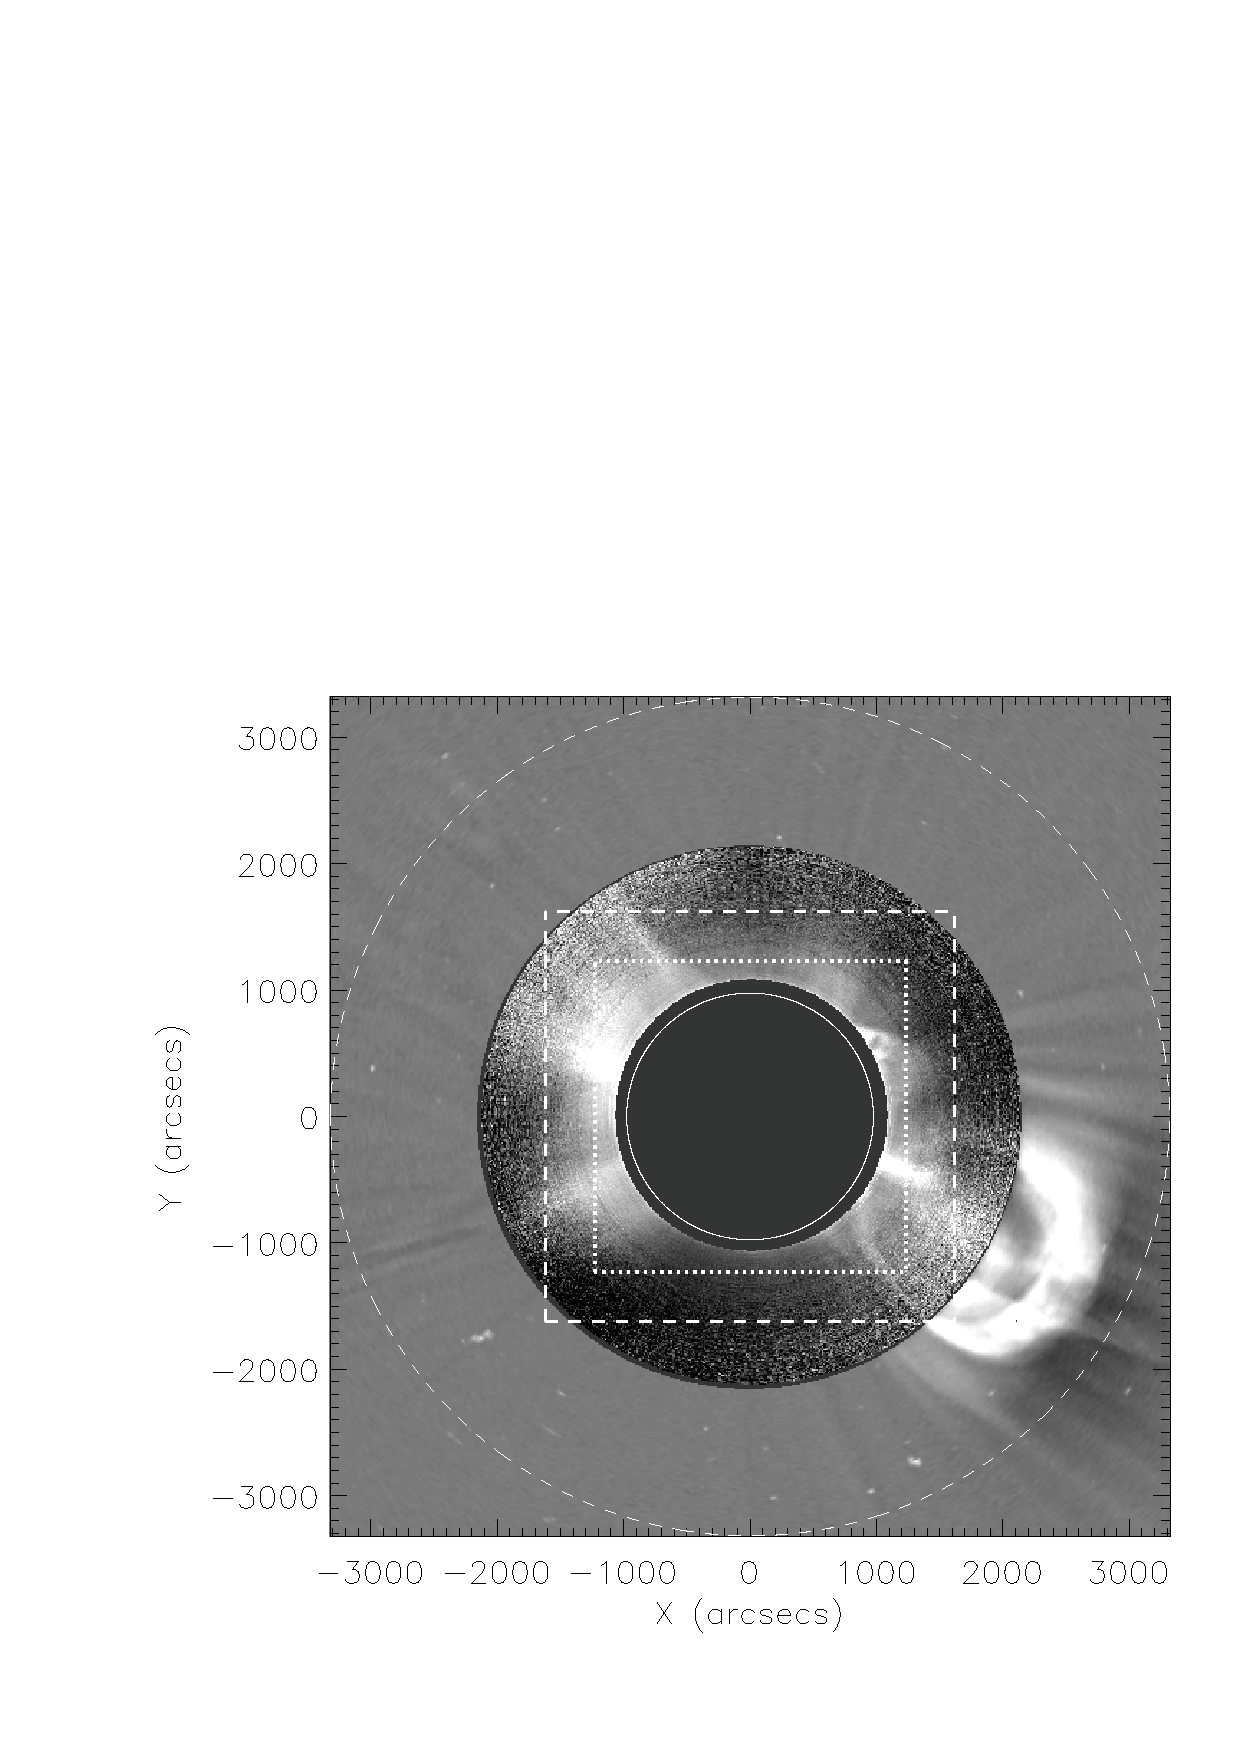
\includegraphics[scale=0.45, trim=60 50 200 70]{images/overlays.pdf}}
%\caption{A LASCO/C2 image with an MLSO/MK4 image overlaid in the range 1.1\,--\,2.2~R$_\odot$, dated 2011 March 8 at 20:24 and 20:22~UT respectively. The C2 image has been processed via the CORIMP techniques of normalising radial graded filter (NRGF) and quiescent background subtraction. It has been trimmed to a half-width of 3.4~R$_\odot$, which is the upper limit of the PROBA2/SWAP FOV as indicated by the dashed circle. The SWAP FOV during nominal operations is indicated by the dashed box. The SDO/AIA FOV is indicated by the inner dotted box. The limb of the Sun behind the occulter is indicated by the solid white circle. A CME is observed off the south-west limb as a bright loop structure with some inner core material, as seen here in the Thomson-scattered white-light coronagraph images. It is clear how the SWAP and AIA images can be used to bridge CME observations to the low corona and solar disk, for studying the physics of their initiation phase.}
%\label{overlays}
%\end{figure}

New CORIMP techniques for detecting and characterizing CMEs in coronagraph data have been developed and applied to the \emph{SOHO}/LASCO and \emph{STEREO}/SECCHI datasets \citep{2012ApJ...752..144M, 2012ApJ...752..145B}, based in part on multiscale methods of image noise suppression and edge enhancement \citep{2009A&A...495..325B, 2008SoPh..248..457Y}. In order to connect CMEs to their source regions, data from disk imagers, such as \emph{PROBA2}/SWAP and \emph{SDO}/AIA, may be used in tandem with the coronagraph observations. However, difficulties in the interpretation of the observed features arise due to the varying instrument specifications, e.g., image passbands, fields-of-view (FOVs), cadences, etc. Therefore, to bridge the gap between the white-light images of the extended corona and the EUV observations of the solar disk and low corona, the SWAP imager was used in conjunction with the MLSO/MK4 coronagraph to directly compare the observations of CMEs as they erupt through the overlapping FOVs. This allows a direct correspondence of features in the EUV images with those in the white-light images, providing new insight into the connection of CMEs to the Sun during their initial phases of eruption and acceleration away from their source regions on the disk.

%\begin{figure}[t]
%\centering{\includegraphics[scale=0.55, trim=65 270 50 300]{images/smaps.pdf}}
%\caption{Combined PROBA2/SWAP and SDO/AIA-171 image of an erupting prominence observed on 2012 April 16 at 17:43~UT. \emph{Left:} The level-1 data, with the AIA image extending to approximately 1.3~R$_\odot$ and SWAP continuing out to $\sim$\,1.7~R$_\odot$. \emph{Right:} The result of a multiscale edge enhancement technique: the intensity showing the relative strengths of the detected edges along the structures in the image. A substantial amount of detail is revealed within the erupting prominence material and across the solar disk and corona.}
%\label{smaps}
%\end{figure}

%\begin{figure*}[ht]
%\centering{\includegraphics[scale=0.39, trim=0 10 0 30]{images/polar_fig_swap.pdf}}
%\caption{The top two panels show polar-unwrapped images of the solar corona across the PROBA2/SWAP FOV on 2012 April 16 at 17:43~UT; left being the level-1 data, right being the enhanced data. Across each image, at a constant height of 1.3~R$_\odot$, an intensity slice is plotted (of arbitrary normalised units) to demonstrate how the background coronal structure is suppressed by the multiscale techniques, to highlight only the complex structure of the prominence. The bottom left plot shows a direct comparison of the two intensity slices, where the prominence is located between 70\,--\,90$^\circ$. The bottom right plot shows a log scale of the normalised intensity slice across the enhanced image to demonstrate that the rest of the coronal structure is still present, just strongly suppressed relative to the prominence material.}
%\label{combine_polar_figs}
%\end{figure*}

\begin{figure}[t]
\centering{\includegraphics[scale=0.15, trim=0 0 0 0]{images/swap_mk4_temp.pdf}}
\caption{SWAP (left) and MK4 (right) observations of the erupting loop system that forms the inner core of the CME on 2011\,March\,8, at times 19:52 and 19:53\,UT respectively. The images have been processed via the multiscale decomposition of \citet{2008SoPh..248..457Y}, showing here intensities that represent the magnitude of the detected edges, at a particular scale with high signal-to-noise ratio.}
\label{swap_front}
\end{figure}

We shall extend the CORIMP techniques, first developed for coronagraphs, to enhance and characterize the detailed structure in the EUV images of SWAP and AIA. For example, an overlay of SWAP and AIA-171 images is shown in Figure~\ref{smaps} for an erupting prominence on 2012 April 16 at 17:43\,UT. The left image shows the level-1 processed data. The right image shows the result of the multiscale filtering technique developed by Young \& Gallagher 2008, applied in such a manner as to enhance the edges of the detected structure in the data. The complex nature of the erupting material is such that its signal may be multiplied across numerous scales, while the more linear background coronal features and small-scale noise fall away (as detailed in Byrne \emph{et al.} 2012). This is demonstrated in Figure~\ref{combine_polar_figs}, where the original and multiscale enhanced SWAP images are polar-unwrapped about Sun-centre and the coronal heights of 1\,--\,1.7\,R$_\odot$ are displayed. The comparison of an intensity slice at a height of 1.3\,R$_\odot$ in each, reveals how the multiscale techniques best characterise the complex structure of the erupting prominence material and suppress the more linear background features. Such methods of image processing will be further enhanced with the application of a radial filter (as per the NRGF technique of Morgan \emph{et al.} 2006 to be extended for use on the EUV images).


The CORIMP methods, which have been used to detect and characterise CMEs in coronagraphs, thus show excellent promise for revealing the structure of the eruptions in EUV images that precede, or underlie, the CMEs. It is a goal of this proposal to develop such techniques for applying to the SWAP images in combination with the MK4 images, to bridge the gap between disk and corona observations. This will allow us to quantify their early acceleration, along with their expansion and possible deflection from their source region locations, in a more comprehensive manner than has been previously possible. These unique datasets will therefore help to advance our knowledge of the forces that act during the initiation phase of CMEs. It is intended that this work be published in a peer-reviewed journal, and the developed codes made publicly available through the CORIMP branch of the SSW tree.


\section{The 8 March 2011 Event}

\begin{figure}[!t]
\centering{\includegraphics[scale=0.35, trim=0 0 0 0, clip=true]{images/xrayflux.png}}
\caption{GOES x-ray flux.}
\label{xrayflux}
\end{figure}

\begin{figure*}[!ht]
\centering
\subfigure[The magnitude of the edge strengths from the multiscale filtering procedure, for an section of the MK4 observation of the erupting CME at 19:56~UT on 8 March 2011. A point-\&-click characterization of the front edge of the CME core material is shown by the plus symbols.]{\includegraphics[clip=true, scale=0.27, trim=60 10 40 10]{images/front_mults.png}}
\label{front_mults}
\subfigure[An MK4 observation of the erupting CME, with the ellipse fit to the points shown in the left figure, in order to characterize the core material of the erupting CME.]{\includegraphics[scale=0.32, clip=true, trim=30 70 70 70]{images/ell_front.png}}
\label{ell_front}
\subfigure[LASCO/C2 observation of the CME at 21:06~UT on 8 March 2011.]{\includegraphics[clip=true, scale=0.32, trim=30 70 70 70]{images/ell_front_c2.png}}
\label{front_mults}
\subfigure[LASCO/C3 observation of the CME at 02:17 on 9 March 2011.]{\includegraphics[scale=0.32, clip=true, trim=30 70 70 70]{images/ell_front_c3.png}}
\label{ell_front}
\caption{MK4 and LASCO observations of a CME as it erupts off the south-west limb on 8 March 2011, with an ellipse fit to the characterized core material.}
\label{mk4_figs}
\end{figure*}

A CME was observed on 2011 March 8 off the west limb, from active region N?? that underwent numerous flares in the preceding hours (Fig.~\ref{xrayflux}). The CME was observed as a series of rising loops, that attained an initial height in the low corona (of approximately half a solar radii) before destabilizing and forming a typical three-part CME structure that propagates out through the corona.

The multiscale filtering technique of \citet{2008SoPh..248..457Y}, as developed for the automated CORIMP CME detection and tracking catalogue \citep{2012ApJ...752..145B}, was employed in the analysis of MK4 and LASCO coronagraph data for the 2011 March 8 event. The filters were applied such that the magnitude of the edge strengths was determined for each image, as shown in Fig.~\ref{mk4_figs}a for a frame at 19:56~UT. This allowed a point-\&-click characterization of the core material of the CME, which was the brightest structure to be tracked through the different imagers when the CME front was not yet fully formed. An ellipse was fit to the detections in order to characterize the dynamical evolution of the CME core throughout the MK4 and LASCO observations.

The kinematic profile of the characterized CME core material is shown in Fig.~\ref{plot_kins_quartiles_all}.

\begin{figure}[ht]
\centering{\includegraphics[scale=0.43, trim=23 10 0 30, clip=true]{images/plot_kins_quartiles_all.pdf}}
\caption{caption.}
\label{plot_kins_quartiles_all}
\end{figure}

\begin{figure}[!t]
\centering{\includegraphics[scale=0.43, trim=23 530 0 30, clip=true]{images/plot_kins_quartiles_inner.pdf}}
\caption{caption.}
\label{plot_kins_quartiles_inner}
\end{figure}

\begin{figure*}[!ht]
\centering
\subfigure{\includegraphics[clip=true, scale=0.26, trim=20 20 20 20]{images/combined.png}}
\label{front_mults}
\subfigure{\includegraphics[scale=0.295, clip=true, trim=10 40 50 50]{images/swap_mk4_ells.png}}
\label{ell_front}
\caption{\emph{Left:} A merged SWAP (blue) and MK4 (red) image with the ellipse fits to the characterized CME core material as observed by each instrument. \emph{Right:} The SWAP and MK4 ellipse fits to the characterized CME core material over the course of the eruption.}
\label{mk4_figs}
\end{figure*}


\section{Conclusions}

%% If you wish to include an acknowledgments section in your paper,
%% separate it off from the body of the text using the \acknowledgments
%% command.

%% Included in this acknowledgments section are examples of the
%% AASTeX hypertext markup commands. Use \url without the optional [HREF]
%% argument when you want to print the url directly in the text. Otherwise,
%% use either \url or \anchor, with the HREF as the first argument and the
%% text to be printed in the second.


\begin{acknowledgements}
This work is supported by SHINE grant 0962716 and NASA grant NNX08AJ07G to the Institute for Astronomy. The \emph{SOHO}/LASCO data used here are produced by a consortium of the Naval Research Laboratory (USA), Max-Planck-Institut fuer Aeronomie (Germany), Laboratoire d'Astronomie (France), and the University of Birmingham (UK). SOHO is a project of international cooperation between ESA and NASA. \emph{SDO} data supplied courtesy of the NASA/\emph{SDO} consortia. The \emph{STEREO}/SECCHI project is an international consortium of the Naval Research Laboratory (USA), Lockheed Martin Solar and Astrophysics Lab (USA), NASA Goddard Space Flight Center (USA), Rutherford Appleton Laboratory (UK), University of Birmingham (UK), Max-Planck-Institut f\"{u}r Sonnen-systemforschung (Germany), Centre Spatial de Liege (Belgium), Institut d'Optique Th\'{e}orique et Appliqu\'{e}e (France), and Institut d'Astrophysique Spatiale (France). The authors would like to acknowledge the help and guidance from the \emph{SDO} Feature Finding Team. DSB was supported by a Marie Curie Intra-European Fellowship under the European Community's Seventh Framework Programme (FP7) and the ESA Prodex program. 
\end{acknowledgements}


%% To help institutions obtain information on the effectiveness of their
%% telescopes, the AAS Journals has created a group of keywords for telescope
%% facilities. A common set of keywords will make these types of searches
%% significantly easier and more accurate. In addition, they will also be
%% useful in linking papers together which utilize the same telescopes
%% within the framework of the National Virtual Observatory.
%% See the AASTeX Web site at http://www.journals.uchicago.edu/AAS/AASTeX
%% for information on obtaining the facility keywords.

%% After the acknowledgments section, use the following syntax and the
%% \facility{} macro to list the keywords of facilities used in the research
%% for the paper.  Each keyword will be checked against the master list during
%% copy editing.  Individual instruments or configurations can be provided 
%% in parentheses, after the keyword, but they will not be verified.


%% Appendix material should be preceded with a single \appendix command.
%% There should be a \section command for each appendix. Mark appendix
%% subsections with the same markup you use in the main body of the paper.

%% Each Appendix (indicated with \section) will be lettered A, B, C, etc.
%% The equation counter will reset when it encounters the \appendix
%% command and will number appendix equations (A1), (A2), etc.


%% The reference list follows the main body and any appendices.
%% Use LaTeX's thebibliography environment to mark up your reference list.
%% Note \begin{thebibliography} is followed by an empty set of
%% curly braces.  If you forget this, LaTeX will generate the error
%% "Perhaps a missing \item?".
%%
%% thebibliography produces citations in the text using \bibitem-\cite
%% cross-referencing. Each reference is preceded by a
%% \bibitem command that defines in curly braces the KEY that corresponds
%% to the KEY in the \cite commands (see the first section above).
%% Make sure that you provide a unique KEY for every \bibitem or else the
%% paper will not LaTeX. The square brackets should contain
%% the citation text that LaTeX will insert in
%% place of the \cite commands.

%% We have used macros to produce journal name abbreviations.
%% AASTeX provides a number of these for the more frequently-cited journals.
%% See the Author Guide for a list of them.

%% Note that the style of the \bibitem labels (in []) is slightly
%% different from previous examples.  The natbib system solves a host
%% of citation expression problems, but it is necessary to clearly
%% delimit the year from the author name used in the citation.
%% See the natbib documentation for more details and options.

\bibliographystyle{apj.bst}
\bibliography{references.bib}  


%% Use the figure environment and \plotone or \plottwo to include
%% figures and captions in your electronic submission.
%% To embed the sample graphics in
%% the file, uncomment the \plotone, \plottwo, and
%% \includegraphics commands
%%
%% If you need a layout that cannot be achieved with \plotone or
%% \plottwo, you can invoke the graphicx package directly with the
%% \includegraphics command or use \plotfiddle. For more information,
%% please see the tutorial on "Using Electronic Art with AASTeX" in the
%% documentation section at the AASTeX Web site,
%% http://www.journals.uchicago.edu/AAS/AASTeX.
%%
%% The examples below also include sample markup for submission of
%% supplemental electronic materials. As always, be sure to check
%% the instructions to authors for the journal you are submitting to
%% for specific submissions guidelines as they vary from
%% journal to journal.

%% This example uses \plotone to include an EPS file scaled to
%% 80% of its natural size with \epsscale. Its caption
%% has been written to indicate that additional figure parts will be
%% available in the electronic journal.


%% Here we use \plottwo to present two versions of the same figure,
%% one in black and white for print the other in RGB color
%% for online presentation. Note that the caption indicates
%% that a color version of the figure will be available online.
%%


%% This figure uses \includegraphics to scale and rotate the still frame
%% for an mpeg animation.


%% If you are not including electonic art with your submission, you may
%% mark up your captions using the \figcaption command. See the
%% User Guide for details.
%%
%% No more than seven \figcaption commands are allowed per page,
%% so if you have more than seven captions, insert a \clearpage
%% after every seventh one.

%% Tables should be submitted one per page, so put a \clearpage before
%% each one.

%% Two options are available to the author for producing tables:  the
%% deluxetable environment provided by the AASTeX package or the LaTeX
%% table environment.  Use of deluxetable is preferred.
%%

%% Three table samples follow, two marked up in the deluxetable environment,
%% one marked up as a LaTeX table.

%% In this first example, note that the \tabletypesize{}
%% command has been used to reduce the font size of the table.
%% We also use the \rotate command to rotate the table to
%% landscape orientation since it is very wide even at the
%% reduced font size.
%%
%% Note also that the \label command needs to be placed
%% inside the \tablecaption.

%% This table also includes a table comment indicating that the full
%% version will be available in machine-readable format in the electronic
%% edition.


%% If the table is more than one page long, the width of the table can vary
%% from page to page when the default \tablewidth is used, as below.  The
%% individual table widths for each page will be written to the log file; a
%% maximum tablewidth for the table can be computed from these values.
%% The \tablewidth argument can then be reset and the file reprocessed, so
%% that the table is of uniform width throughout. Try getting the widths
%% from the log file and changing the \tablewidth parameter to see how
%% adjusting this value affects table formatting.

%% The \dataset{} macro has also been applied to a few of the objects to
%% show how many observations can be tagged in a table.


%% Tables may also be prepared as separate files. See the accompanying
%% sample file table.tex for an example of an external table file.
%% To include an external file in your main document, use the \input
%% command. Uncomment the line below to include table.tex in this
%% sample file. (Note that you will need to comment out the \documentclass,
%% \begin{document}, and \end{document} commands from table.tex if you want
%% to include it in this document.)

%% \input{table}

%% The following command ends your manuscript. LaTeX will ignore any text
%% that appears after it.

\end{document}

%%
%% End of file `sample.tex'.
